\subsection{New definitions}
\label{sec:New definitions}
We define the concept of a vel inductively:
\begin{definition}
  We say that two nodes $a,b$ are connected by a \textbf{vel} ($V(a,b)$) if:
  \begin{itemize}
    \item (BC $\rightarrow$) $b \in N(a)$.
    \item (BC $\leftarrow$) $a \in N(b)$.
    \item (IS $\rightarrow$) ($\exists c \in N(a))[( \forall x \in N(c))(V(x,b) \vee V(x,x) \vee V(x,a))]$\todo{We need at least one of the V(x,b) to exist.}
      \item (IS $\leftarrow$) ($\exists c \in N(b))[( \forall x \in N(c))(V(x,a) \vee V(x,x) \vee V(x,b))]$
  \end{itemize}
\end{definition}
We can illustrate the different cases with the following figures (with dashed lines representing vels):
\[
  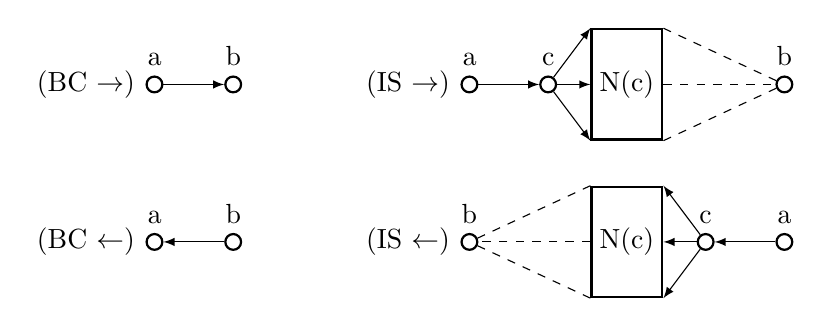
\begin{tikzpicture}
    [
    point/.style={thick,circle,draw,inner sep=0pt,minimum size=2mm},
    collection/.style={thick,rectangle,draw,inner sep=0pt,minimum height=14mm, minimum width= 9mm}
    ]
    \node (label) at (1,2) [label=left:(BC $\rightarrow$)] {};
    \node (0) at (1,2) [point,label=above:a] {};
    \node (1) at (2,2) [point,label=above:b] {};
    \draw [-latex] (0) to (1);

    \node (label) at (1,0) [label=left:(BC $\leftarrow$)] {};
    \node (0) at (1,0) [point,label=above:a] {};
    \node (1) at (2,0) [point,label=above:b] {};
    \draw [-latex] (1) to (0);

    \node (label) at (5,2) [label=left:(IS $\rightarrow$)] {};
    \node (0) at (5,2) [point,label=above:a] {};
    \node (1) at (6,2) [point,label=above:c] {};
    \node (2) at (7,2) [collection,label=center:N(c)] {};
    \node (3) at (9,2) [point,label=above:b] {};
    \draw [-latex] (0) to (1);
    \draw [-latex] (1) to (2.north west);
    \draw [-latex] (1) to (2.west);
    \draw [-latex] (1) to (2.south west);
    \draw [-, dashed] (2.north east) to (3);
    \draw [-, dashed] (2.east) to (3);
    \draw [-, dashed] (2.south east) to (3);

    \node (label) at (5,0) [label=left:(IS $\leftarrow$)] {};
    \node (0) at (9,0) [point,label=above:a] {};
    \node (1) at (8,0) [point,label=above:c] {};
    \node (2) at (7,0) [collection,label=center:N(c)] {};
    \node (3) at (5,0) [point,label=above:b] {};
    \draw [-latex] (0) to (1);
    \draw [-latex] (1) to (2.north east);
    \draw [-latex] (1) to (2.east);
    \draw [-latex] (1) to (2.south east);
    \draw [-, dashed] (2.north west) to (3);
    \draw [-, dashed] (2.west) to (3);
    \draw [-, dashed] (2.south west) to (3);
  \end{tikzpicture}
\]

Note that both the base case and the inductive step is given in symmetric pairs, making $V$ a symmetric relation: $V(a,b) \Leftrightarrow V(b,a)$.
\begin{definition}
  A path is a directed version of the vel.  Its definition consists of (BC $\rightarrow$) and (IS $\rightarrow$) from above.
\end{definition}
\begin{lemma}
  If there is a vel between the two nodes $a$ and $b$ and $b$ has no outgoing edges contained in the vel, then the vel is a path going from $a$ to $b$.
\end{lemma}
Assuming a vel between two nodes, we overload the notation and let $V(a,b)$ be the set of edges contained in the vel.  This is obviously only well-defined when the vel in question actually exists.  We can now write the above lemma formally as:
\begin{align*}
  V(a,b) \cap N(b) = \emptyset \quad \Rightarrow \quad P(a,b)
\end{align*}
\begin{proof}
  TODO
\end{proof}
We will show that paths can be constructed in several ways, and we will define a more general way to construct vels using paths.  This will lead to
\begin{lemma}
  If there is a vel between two nodes $a$ and $b$ such that all neighbors of $a$ contained\todo{We need a precise notion of what it means for an edge/node to be contained in a vel} in the vel also has vels to $b$, then there is a vel between $b$ and $b$.
\end{lemma}
\begin{align*}
  ((\forall c \in V(a,b) \cap N(a))(V(c,b))) \Rightarrow V(b,b)
\end{align*}
This is a property purely on the vel structure, so we prove it using structural induction on the vel $V(a,b)$.
\begin{proof}
  (BC $\rightarrow$) In this case, the only neighbor of $a$ contained in the vel is $b$.  Since we assume that all neighbors of $a$ has a vel to be, we immediately get $V(b,b)$.

  (BC $\leftarrow$) In this case $a$ has no neighbors, so our statement becomes vacuously true.

  (IS $\rightarrow$) Referring to our illustration of this situation, our assumption gives us $V(a,b)$ and $V(c,b)$.  By the definition of a vel, we have that for each $x \in N(c)$, either $V(x,b)$, $V(x,x)$ or $V(x,a)$. Since we assume $V(c,b)$, we also get that there is a node $x_i$ in $N(c)$ such that for all $y \in N(x_i)$, we get that either $V(y,b)$, $V(y,y)$ or $V(y, )$.
\end{proof}
\pagebreak
